\documentclass{beamer}
\usepackage{graphics}
\title{Using the  AJIT Application Development Environment}
\author{Madhav P. Desai, Anshuman Dhuliya, Gauri Patrikar}
\begin{document}
\maketitle

\frame[containsverbatim]{\frametitle{Overview}
%\begin{figure}
  %\centering
  %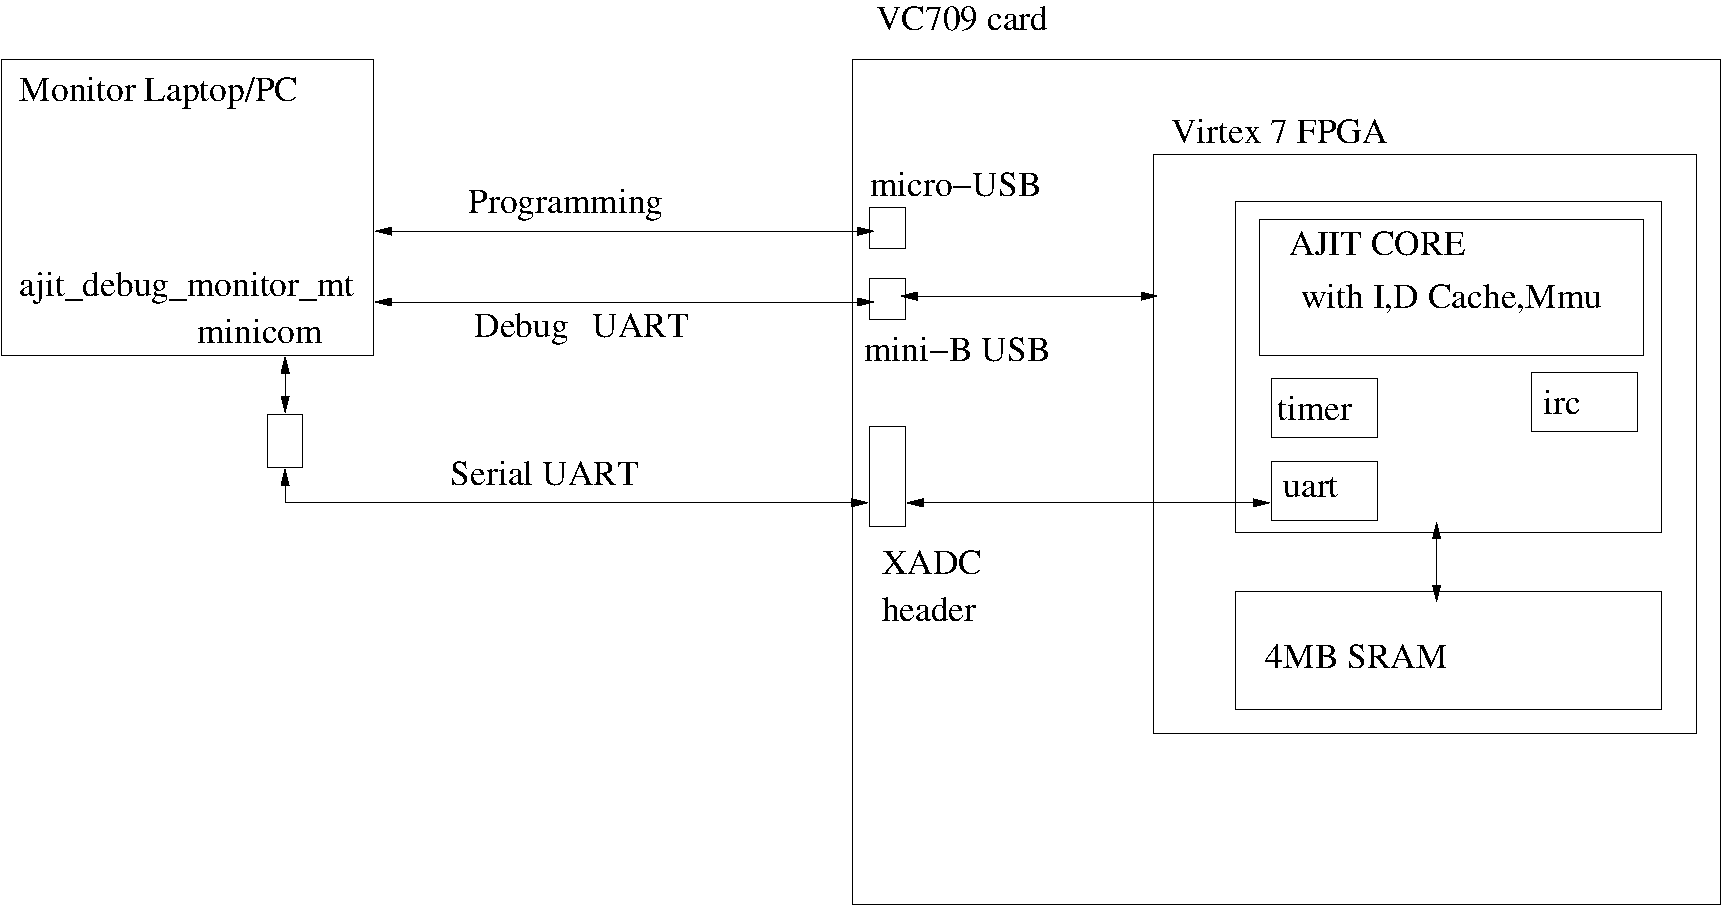
\includegraphics[width=10cm]{figs/vc709Setup.pdf}
  %\caption{AJIT single board computer on VC709}
%\end{figure}

\begin{itemize}

\item The AJIT platform.
\begin{itemize}
\item The processor.
\item Memory map:  Flash, RAM, Non-cacheable RAM, IO.
\item Peripherals: Serial UART, Timer, Interrupt Controller, SPI Master, I2C Master.
\end{itemize}
\item The development environment and support system.
\begin{itemize}
\item CORTOS-2.
\item AJIT access routines, minimal print and timer routines.
\item Flash image creation utility.
\end{itemize}
\item The User Application.
\begin{itemize}
\item User code.
\item Interrupt service routines.
\item Software trap handlers.
\item Locks, dynamic memory allocation.
\end{itemize}
\end{itemize}

}

\frame[containsverbatim]{\frametitle{The AJIT platform model}
\begin{figure}
  \centering
  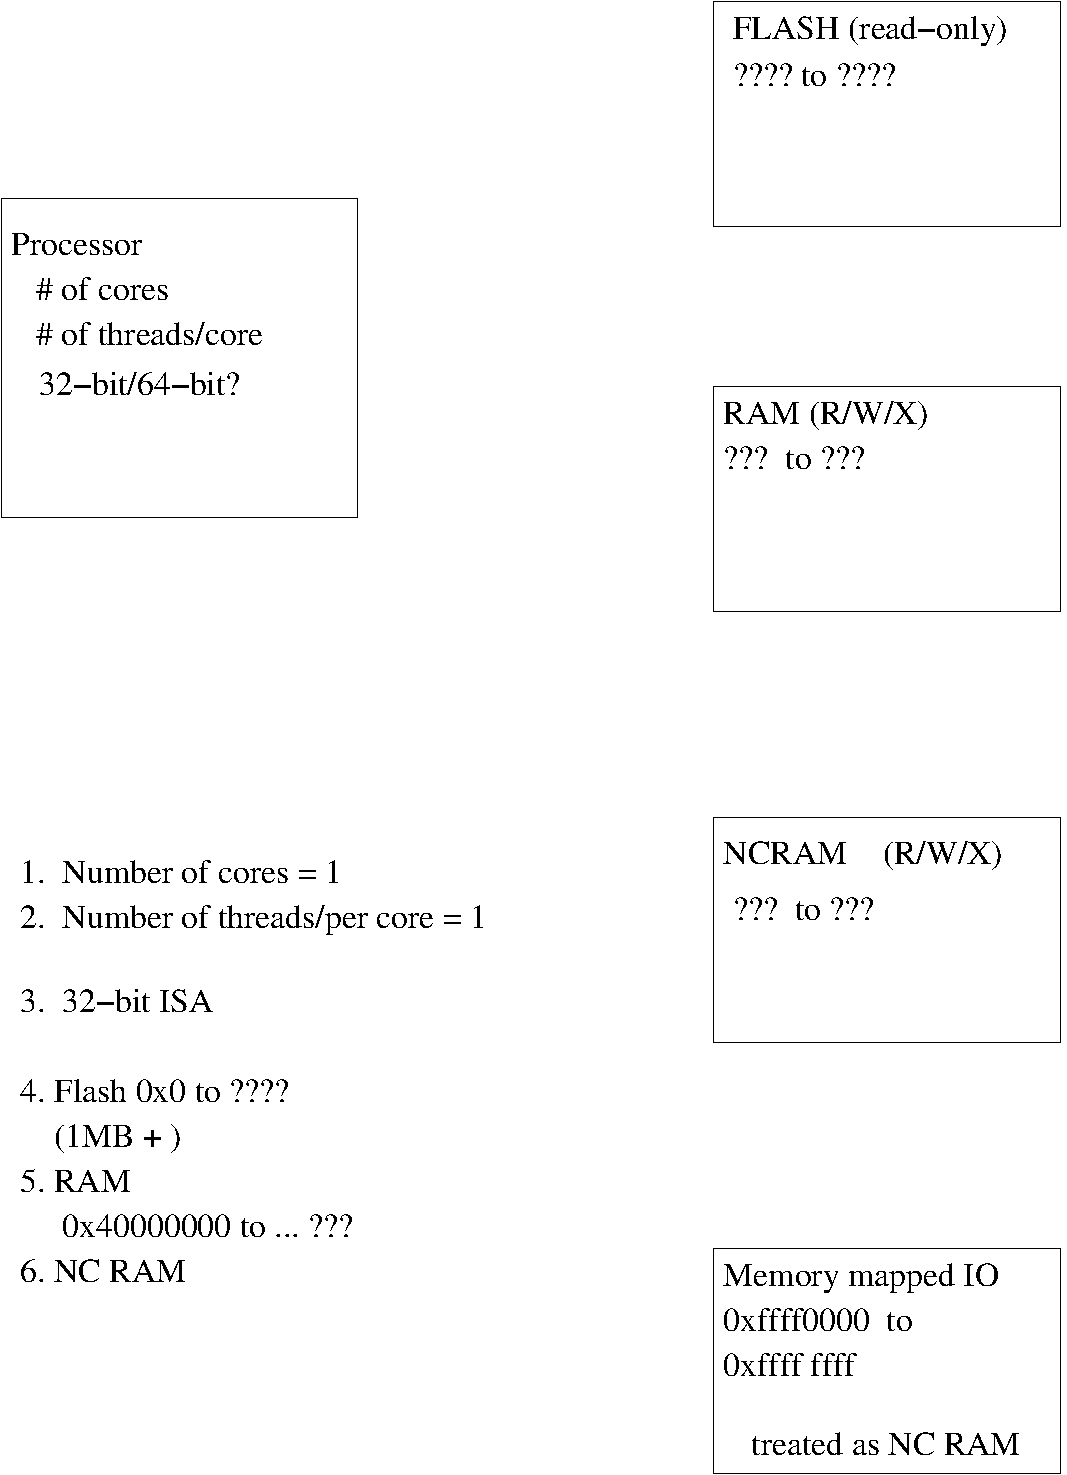
\includegraphics[width=5cm]{figs/Platform.pdf}
  \caption{The AJIT platform model}
\end{figure}
}

\frame[containsverbatim]{\frametitle{The AJIT platform model: Recap}
\begin{itemize}
\item The processor.
\item The memory regions.
\begin{itemize}
\item The FLASH region.
\item The RAM region.
\item The non-cacheable (NC) RAM region.
\item The IO region.
\end{itemize}
\item Platform can be described to development environment 
using a CORTOS2 configuration file.
\end{itemize}
}

\frame[containsverbatim]{\frametitle{CORTOS-2 configuration file: abstraction of the AJIT platform model, and specification of software}

\begin{verbatim}
Hardware:
  Processor:
    # Required: Number of cores and threads per core.
    Cores: 1
    ThreadsPerCore: 1
    ISA: 32 # 32/64 bit (Default: 32)
\end{verbatim}

}

\frame[containsverbatim]{\frametitle{CORTOS-2 configuration file: platform description continued.}
\begin{verbatim}
  Memory:
    MaxPhysicalAddrBitWidth: 36
    Flash:
      StartAddr: 0x0  # physical address
      SizeInMegaBytes: 16
      Permissions: RXC  # (Read,Write,eXecute,Cacheable)
    RAM:
      StartAddr: 0x40000000
      SizeInMegaBytes: 128
      Permissions: RWXC
    NCRAM:
      StartAddr: 0x8000000
      SizeInMegaBytes: 16
      Permissions: RW
    MMIO: # Memory Mapped IO
      StartAddr: 0xFFFF0000  # physical address
      EndAddr:   0xFFFFFFFF
      Permissions: RW
\end{verbatim}
}
\frame[containsverbatim]{\frametitle{CORTOS-2 configuration file: platform description continued.}
\begin{verbatim}
  # see ./AjitPublicResources/tools/ajit_access_routines_mt/include/device_addresses.h
  Devices:
    - Name: Timer
      MemoryRegion:
        StartAddr: 0xFFFF3100 # physical address (in MMIO)
        SizeInBytes: 256 # 16x16
        Permissions: RW
      NamedRegisters:
        Control: 0xFFFF3100
    - Name: InterruptController
      MemoryRegion:
        StartAddr: 0xFFFF3000
        SizeInBytes: 32
        Permissions: RW
      NamedRegisters:
        Control: 0xFFFF3000
\end{verbatim}
}
\frame[containsverbatim]{\frametitle{CORTOS-2 configuration file: platform description continued.}
\begin{verbatim}
    - Name: Serial
      MemoryRegion:
        StartAddr: 0xFFFF3200
        SizeInBytes: 64
        Permissions: RW
      NamedRegisters:
        Control: 0xFFFF3200
        TX: 0xFFFF3204
        RX: 0xFFFF3208
    - Name: ScratchArea
      MemoryRegion:
        StartAddr: 0xFFFF2C00
        SizeInBytes: 1024
        Permissions: RW
\end{verbatim}
}
\frame[containsverbatim]{\frametitle{CORTOS-2 configuration file: software description}
\begin{verbatim}
Software:
  BuildAndExecute:
    LogLevel: DEBUG
    OptimizationLevel: 2 # i.e. O2 (Accepted values: 0, 1, 2)
    EnableSerial: Yes # Yes/No (Default: Yes)
    Debug: No # Yes/No (Default: No)
    FirstDebugPort: 8888
    BuildArgs: "-D CORTOS_ENV"
  ProgramThreads:
    - CortosInitCalls:
        - main
      StackSize:
        SizeInKiloBytes: 16
  DynamicMemory: # Dynamic Memory Configuration.
    SizeInKiloBytes: 1000
\end{verbatim}
}

\frame[containsverbatim]{\frametitle{CORTOS-2 configuration file: software description}
Other things that the user can provide are
\begin{itemize}
\item interrupt handlers for each interrupt level.
\item software trap handlers for ta 1 to to ta 15.
\end{itemize}
}

\frame[containsverbatim]{\frametitle{CORTOS-2 configuration file: Summary}
In one file, we have specified:
\begin{itemize}
\item The platform.
\item The software:
\begin{itemize}
\item The single thread in the system, will jump to function main after initialization
of the thread.
\item The user does not need to worry about the details of the initialization.
\end{itemize}
\end{itemize}
}

\frame[containsverbatim]{\frametitle{CORTOS-2 resources, and what it does}

\begin{itemize}
\item queues.
\item locks, both cacheable and non-cacheable.
\item dynamic memory allocation: both cacheable and non-cacheable.
\item logging.
\item thread safe printing.
\item CORTOS functionality:
\begin{itemize}
\item Figures out memory requirements by the user application.
\item Identifies memory for stacks, queues, locks, non-cacheable locks.
\item Generates VA->PA mapping code as part of initialization.
\item Sets up interrupt and trap handlers as indicated by the user.
\end{itemize}
\end{itemize}

}


\frame[containsverbatim]{\frametitle{Programming resources: AJIT access routines}

Located in
\begin{verbatim}
AjitPublicResources/tools/ajit_access_routines_mt
   include/
   src/
   asm/
\end{verbatim}

Lots of useful routines.  Used seamlessly by CORTOS2,
with user intervention not required in most cases.

}

\frame[containsverbatim]{\frametitle{Programming resources: Minimal print, timer functions}
\begin{verbatim}
AjitPublicResources/tools/minimal_printf_timer
   include/
   src/
\end{verbatim}
}

\frame[containsverbatim]{\frametitle{Initialization code generated by CORTOS2}

\begin{itemize}
\item Clear the stack pointers.
\item Setup PSR, WIM registers
\item Setup Virtual to Physical mapping page table in memory.
\item Jump to user main.
\end{itemize}

NOTE:  This is handled by the CORTOS2 build framework and
user intervention is not necessary.
}


\frame[containsverbatim]{\frametitle{Exceptions}

\begin{itemize}
\item Hardware traps.
\item Software traps.
\item Interrupts.
\end{itemize}

}


\frame[containsverbatim]{\frametitle{Hardware traps}
\begin{itemize}
\item With existing trap handlers:
\begin{itemize}
\item Window overflow trap (trap 0x5). 
\item Window underflow trap (trap 0x6).
\end{itemize}
\item With default trap handlers (processor goes into error):
\begin{itemize}
\item Instruction access exception (0x1).
\item Invalid Instruction trap (0x2).
\item Privileged Instruction trap (0x3).
\item FP disabled trap (0x4).
\item Unaligned access trap (0x7).
\item Floating point exception (0x8).
\item Data access exception (0x9).
\item Tag overflow trap (0xa).
\item Coprocessor disabled trap (0x24).
\item Integer divide by zero (0x2A).
\end{itemize}
\end{itemize}

}

\frame[containsverbatim]{\frametitle{Software traps}

\begin{itemize}

\item ta [0-127].
\item ta 0 is reserved.
\item ta 1-15 available for user code.
\item User can write own trap handlers for each of these traps.
\item CORTOS2 will setup trap chain seamlessly.
\end{itemize}

}

\frame[containsverbatim]{\frametitle{Interrupts}
\begin{itemize}

\item 15 interrupt levels.
\item Interrupt handler can be provided by the user for each interrupt level.
\item CORTOS2 will setup interrupt handler chain seamlessly.

\end{itemize}

}


\frame[containsverbatim]{\frametitle{Next Steps}
\begin{itemize}
\item Work out individual examples highlighting CORTOS2 capabilities.
\begin{itemize}
\item Single-core single-thread processor (provided to SAC).
\item Using queues.
\item Using locks.
\item Using dynamic memory allocation (cacheable/non-cacheable).
\item Setting up interrupt handlers.
\item Setting up software trap handlers.
\end{itemize}
\item Debugging and AJIT debug monitor.
\item Flash image preparataion.
\item Using the peripherals.
\item If interested, Multi-core and multi-thread processors.
\end{itemize}
}

\end{document}


